\documentclass[11pt]{report}
\usepackage[a4paper]{geometry}
\usepackage[myheadings]{fullpage}
\usepackage{fancyhdr}
\usepackage{lastpage}
\usepackage{graphicx, wrapfig, subcaption, setspace, booktabs}
\usepackage[T1]{fontenc}
\usepackage[font=small, labelfont=bf]{caption}
\usepackage[protrusion=true, expansion=true]{microtype}
\usepackage{sectsty}
\usepackage{url, lipsum}
\usepackage{mathptmx}
\usepackage[utf8]{inputenc}
\usepackage[francais]{babel}
\pagestyle{plain}

\newcommand{\HRule}[1]{\rule{\linewidth}{#1}}
\onehalfspacing
\setcounter{tocdepth}{5}
\setcounter{secnumdepth}{5}

\renewcommand{\thesection}{\arabic{section}}

%-------------------------------------------------------------------------------
% TITLE PAGE
%-------------------------------------------------------------------------------

\begin{document}

\title
{
	\Large{Cahier des charges}
	\HRule{2pt} \\ [0.5cm]
	\LARGE \textbf{\uppercase{Bacchanight}}
	\HRule{2pt} \\ [0.5cm]
	\normalsize \today
}

\date{}

\author
{
	\LARGE{Université de Bordeaux} \\
	\\
	Alexandre CASANOVA FRANGER \\
	Guillaume CHARLET \\
    Kenji FONTAINE \\
    Gauthier LAMARQUE \\
	Ny Andry RAHARISON \\
}

\maketitle

%-------------------------------------------------------------------------------
% Présentation du projet + Besoins fonctionnels
%-------------------------------------------------------------------------------

\renewcommand{\thesection}{\arabic{section}}

\section{Présentation}

La Baccha-night, du mot « bacchanales », fêtes mythologiques en l’honneur du dieu du vin Bacchus, est un évènement nocturne étudiant proposé par le musée des Beaux-Arts de Bordeaux le mardi 21 mars 2017.
Le but de ce projet est d'élaborer un outil permettant de mieux renseigner les internautes sur la soirée (programme, accès, réseaux sociaux, etc.).

\section{Besoins fonctionnels}

Le site doit utiliser le même système de gestion du contenu que le site actuel
du Musée des Beaux Arts : \textbf{Drupal 7}. \\

Le site doit permettre l'accès aux informations suivantes :
\begin{itemize}
	\item Description de la soirée,
	\item Date et lieu,
	\item Programme/Planning de la soirée,
	\item Historique des sessions précédentes,
	\item Plan d'accès Google Maps,
	\item Contact, lien vers les réseaux sociaux du Musée des Beaux Arts.
\end{itemize}

\vspace{0.5cm}

L'ensemble des informations ci-dessus doit être modifiable par une personne
ayant accès au CMS Drupal. \\

\begin{itemize}
	\item La description est un champ texte modifiable via Drupal.
	\item La date et le lieu seront inclus dans la description.
	\item Le programme/planning est un champ texte qui sera modifiable via Drupal.
	\item L'historique des sessions précédentes est représenté par un carousel
	(module Drupal) montrant des images des événements passés.
	\item Le plan d'accès Google Maps est fait par un module de Drupal.
	L'adresse est modifiable en utilisant le module.
	\item Les liens vers les réseaux sociaux sont fait par des boutons/icones,
	crées et modifiables via un module Drupal.
	\item L'ensemble de ces éléments peuvent être réarrangés dans n'importe quel ordre grâce au système de blocs de Drupal.
\end{itemize}

\subsection*{Hébergement}
Prise de contact avec la Mairie de Bordeaux, actuellement chargée de
l'hébergement du site du Musée des Beaux-Arts.

\subsection*{Déploiement}
Création de la page en utilisant le système de gestion de contenu Drupal
(version 7) déjà présent sur le site du Musée des Beaux-Arts.
Un manuel permettant à une personne ayant de l'expérience avec Drupal
d'intégrer le site au site actuel du musée devra être fourni.

%-------------------------------------------------------------------------------
% Besoins non fonctionnels
%-------------------------------------------------------------------------------

\section{Besoins non fonctionnels}

\subsection*{Charte graphique}

En ce qui concerne la charte graphique, le musée des Beaux Arts de Bordeaux nous a transmis un document (disponible en annexe) regroupant tous les éléments graphiques (images, polices, logos, etc.) que nous avons intégrés au site.

Le site est sous un format One Page. Un site One Page est un site constitué
d'une seule et même page sur laquelle l'ensemble des informations du site web
est disponible en scrollant (ou à l'aide d'une barre de navigation).

\subsection*{Accessibilité}

Le site doit être accessible à partir des navigateurs suivants (toutes plateformes confondues):
%% Ajouter les numéros de versions.
\begin{center}
	\begin{tabular}{|l | r|} 
		\hline
		Navigateurs & Parts de marché \\ 
		\hline
		\hline
		Google Chrome 54+ & 51\%  \\ 			
		\hline
		Mozilla Firefox 51.0+ & 7,4\% \\		
		\hline
		Safari (Apple) 10.0+ & 18,3\% \\ 
		\hline
		Microsoft Edge / IE 11.0 & 10,8\% \\
		\hline
	\end{tabular}
\end{center}
Ces navigateurs ont été sélectionnés à partir de leur pourcentage de parts de marché (toutes supérieures à 5\%). Ce pourcentage est une moyenne des pourcentages recueillis sur les sites suivants:
\begin{itemize}
	\item StatCounter
	\item Net MarketShare
	\item W3Counter
	\item Akamai
\end{itemize}

\subsection*{Responsive}
Puisque le site doit être accessible depuis plusieurs plateformes, le site doit s'adapter à la taille de l'écran.

\subsection*{Léger}
Le site doit se charger en moins de X secondes, en utilisant une connection à
X ko/s. (à tester)

%-------------------------------------------------------------------------------
% Retro planning
%-------------------------------------------------------------------------------

\section{Retro planning}

\begin{itemize}
	\item Version statique pour avant le 21 Mars. (priorité haute)
	\item Version pérenne pour la fin du semestre. (mi-Avril, à confirmer)
\end{itemize}

%-------------------------------------------------------------------------------
% Maquette
%-------------------------------------------------------------------------------

\newpage

\section{Annexe : Maquette}

\vspace{0.4cm}
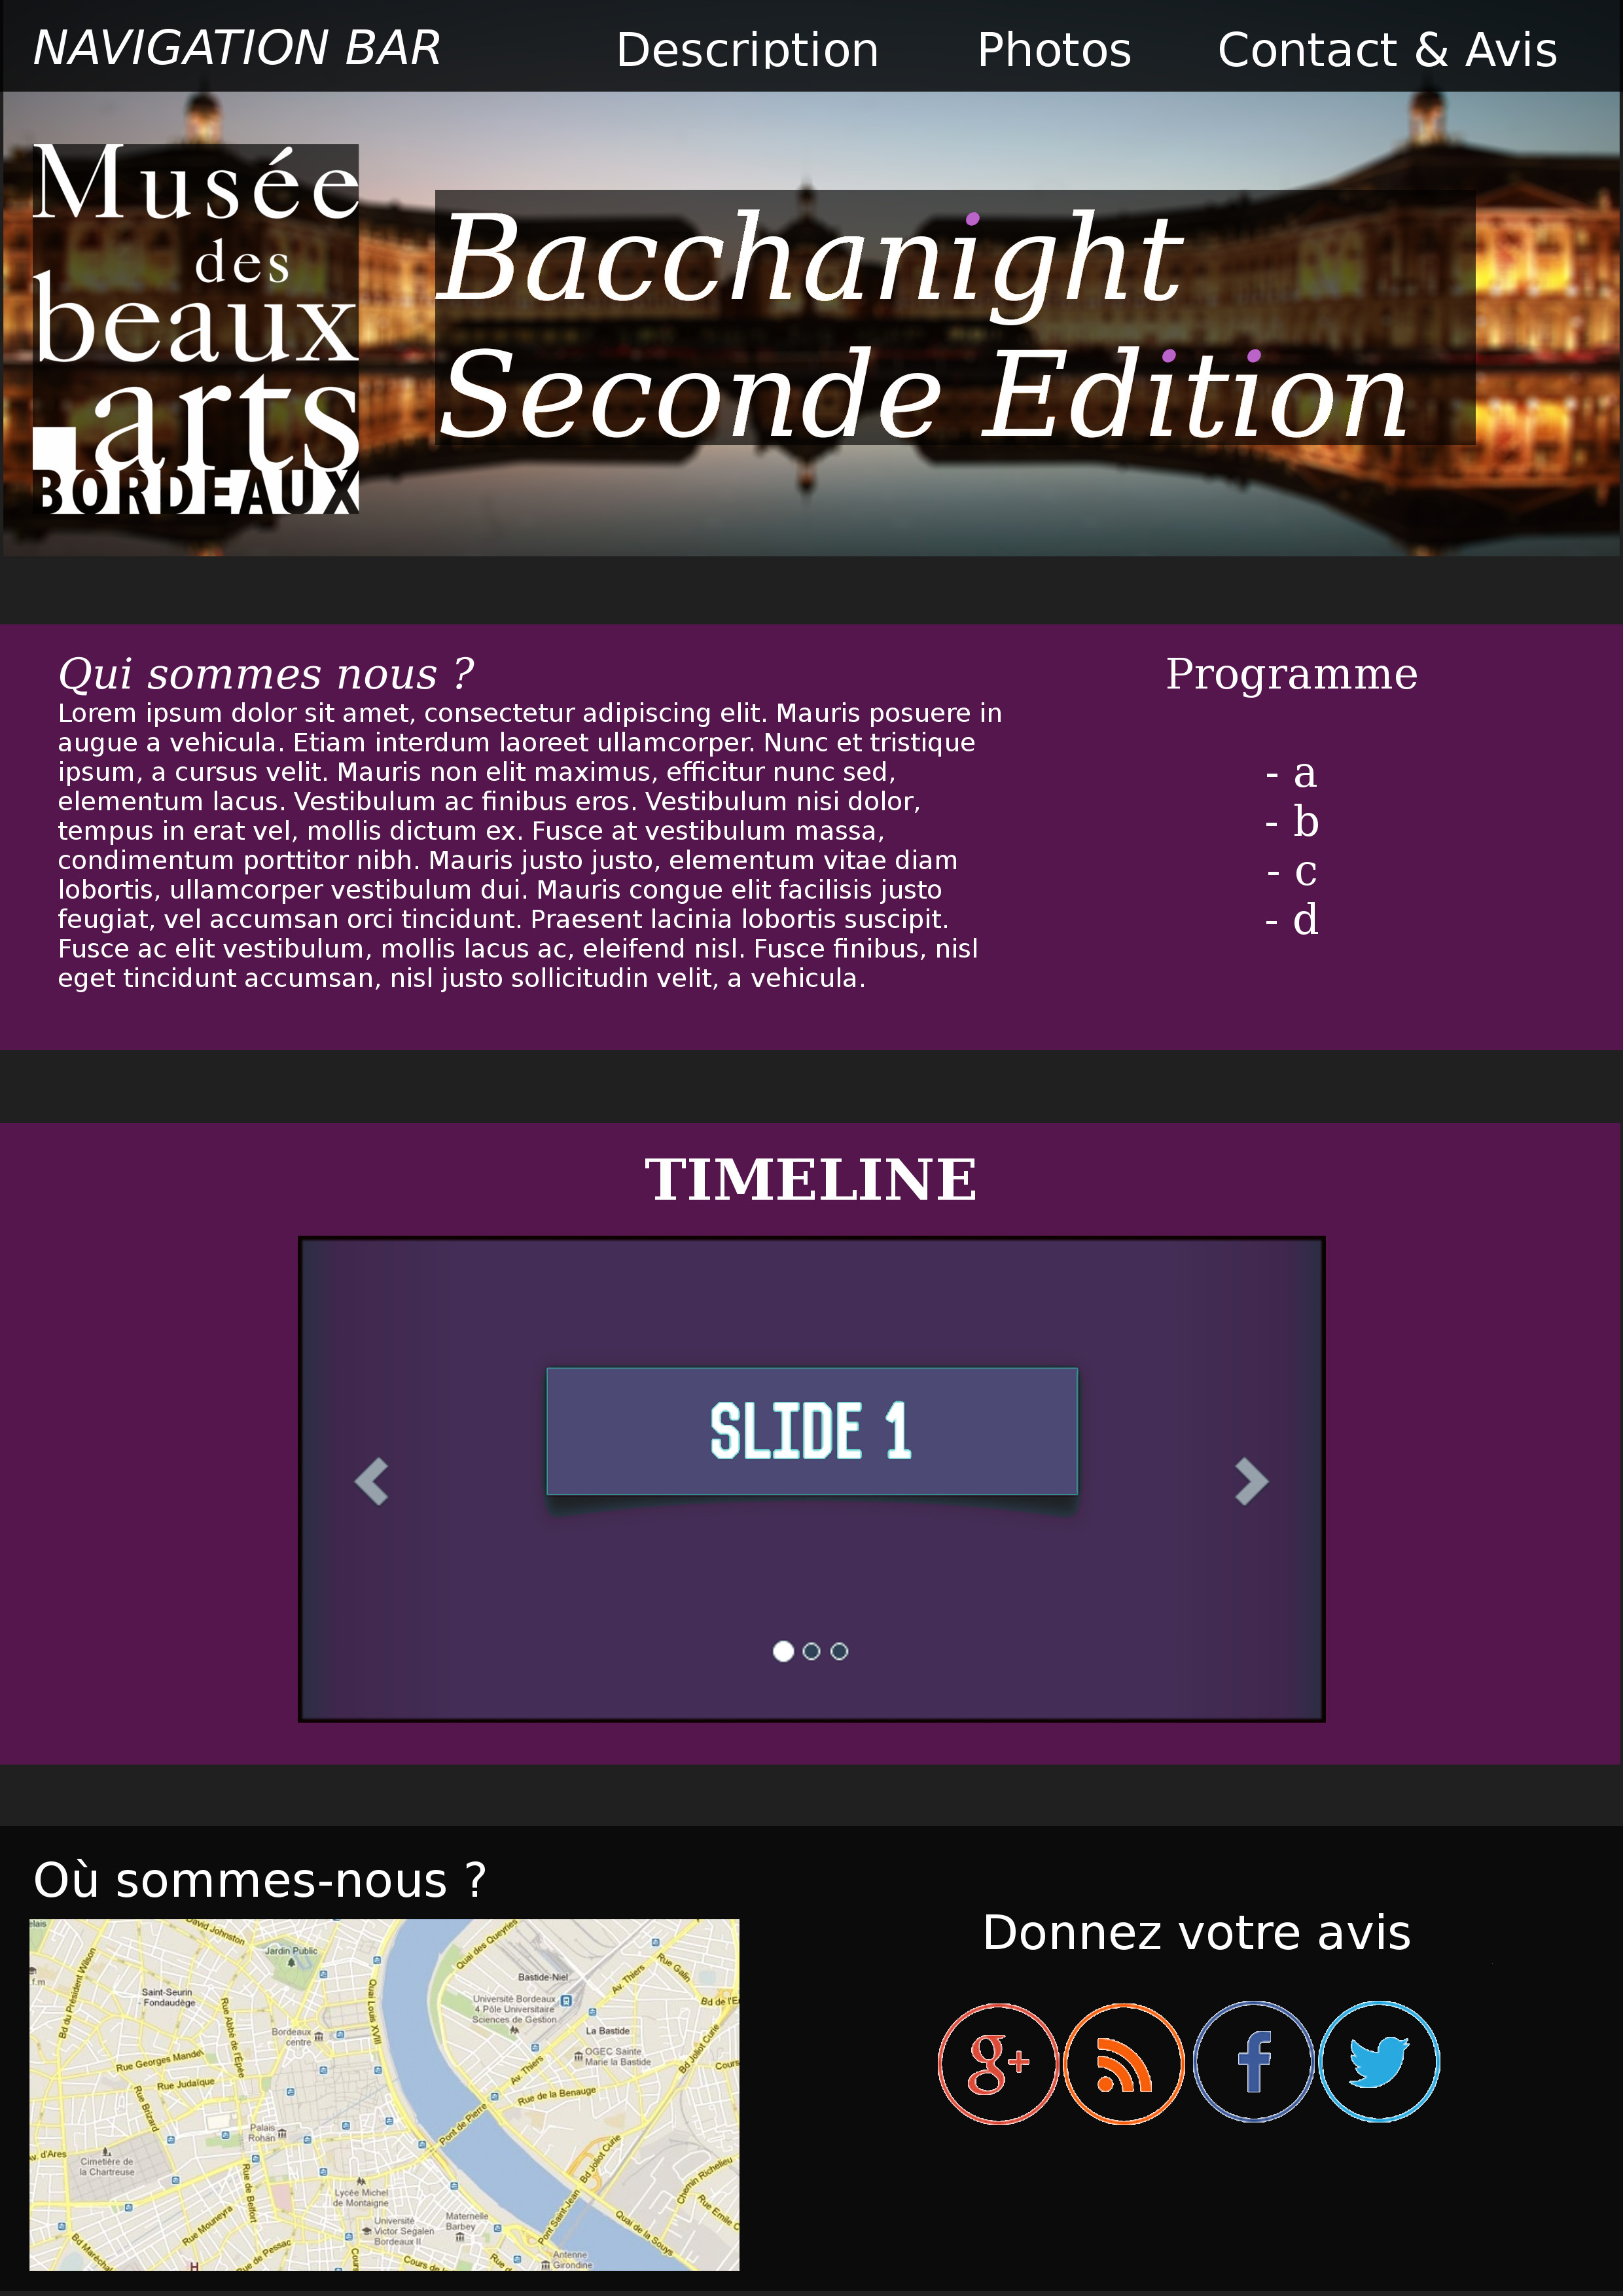
\includegraphics[scale=0.75]{maquette.jpg}

\end{document}
